\chapter[Alocação de Tarefas em Sistemas Multi-Robôs]{Alocação de Tarefas em Sistemas Multi-Robôs} \label{cap:cap3}
    Colocar texto aqui 
    
    % 1a seção do capítulo 3
    \section{Definição Formal} \label{sec:sec3_1}
    Colocar texto aqui
    
    % 2a seção do capítulo 3
    \section{Taxonomias} \label{sec:taxonomias}
        
        \citeonline{ref:gerkey2004taxonomy} sugeriram uma taxonomia independente do domínio de três eixos para a classificação de problemas de alocação de tarefas em sistemas multi-robôs. 
        
        O primeiro eixo determina o \textit{tipo dos robôs} que compõem o problema. Os tipos de robôs possíveis são: \textit{ST} (acrônimo para \textit{Single-Task}) e \textit{MT} (acrônimo para \textit{Multi-Task}). Problemas que envolvem robôs que só podem executar uma tarefa por vez são compostos por robôs do tipo \textit{ST}. Entretanto, se houver pelo menos um robô capaz de executar mais de uma tarefa simultaneamente, então esse problema é composto por robôs do tipo \textit{MT}. 
        
        O segundo eixo da taxonomia determina o \textit{tipo das tarefas} que compõem o problema. Nesse caso, são possíveis os tipos: \textit{ST} (acrônimo para \textit{Single-Robot} e \textit{MR} (acrônimo para \textit{Multi-Robot}). Problemas cujo tipo das tarefas é \textit{SR}, diz-se que todas as tarefas envolvidas só podem ser executadas por um robô. Porém, quando o tipo das tarefas envolvidas é \textit{MR}, diz-se que existe tarefas que podem ser executadas por mais de um robô.
        
        O terceiro eixo, por sua vez, determina o \textit{tipo da alocação} do problema, o qual pode assumir os valores: \textit{IA} (acrônimo para \textit{Instantaneous Assignment}) ou \textit{TA} (acrônimo para \textit{Time-extended Assignment}). O primeiro caso, \textit{IA}, diz repeito à problemas MRTA onde as alocações das tarefas para os robôs são realizadas instantaneamente, sem levar em consideração o estado futuro do sistema. Por outro lado, em problemas cujo tipo de alocação é \textit{TA}, além de conhecido o estado atual de cada rôbo e do ambiente, também é conhecido o conjunto de tarefas que precisarão ser alocadas no futuro. Neste último caso, diversas tarefas são alocadas para um robô, o qual deve executar cada alocação conforme seu agendamento. De acordo com \cite{ref:bastos2008utility}, quando o tipo de alocação do problema MRTA é \textit{IA}, o número de robôs é superior ao número de tarefas alocadas e quando \textit{TA}, o oposto acontece. Isso se deve ao fato de que, em problemas MRTA cujo tipo de alocação é \textit{IA}, o número de robôs no sistema é capaz de suprir a taxa de tarefas a serem atribuídas, de modo que é muito provável que haverão robôs ociosos no sistema; enquanto, naqueles cujo tipo de alocação é \textit{TA}, o número de robôs que compõem o sistema não é suficiente para atender a taxa de tarefas a serem alocadas no sistema.
        
        \begin{figure}[htb]
            \centering
            % Graphic for TeX using PGF
% Title: ../figures/taxonomia_mrta.dia
% Creator: Dia v0.97.2
% CreationDate: Tue Oct 17 17:33:09 2017
% For: adrianohrl
% \usepackage{tikz}
% The following commands are not supported in PSTricks at present
% We define them conditionally, so when they are implemented,
% this pgf file will use them.
\ifx\du\undefined
  \newlength{\du}
\fi
\setlength{\du}{15\unitlength}
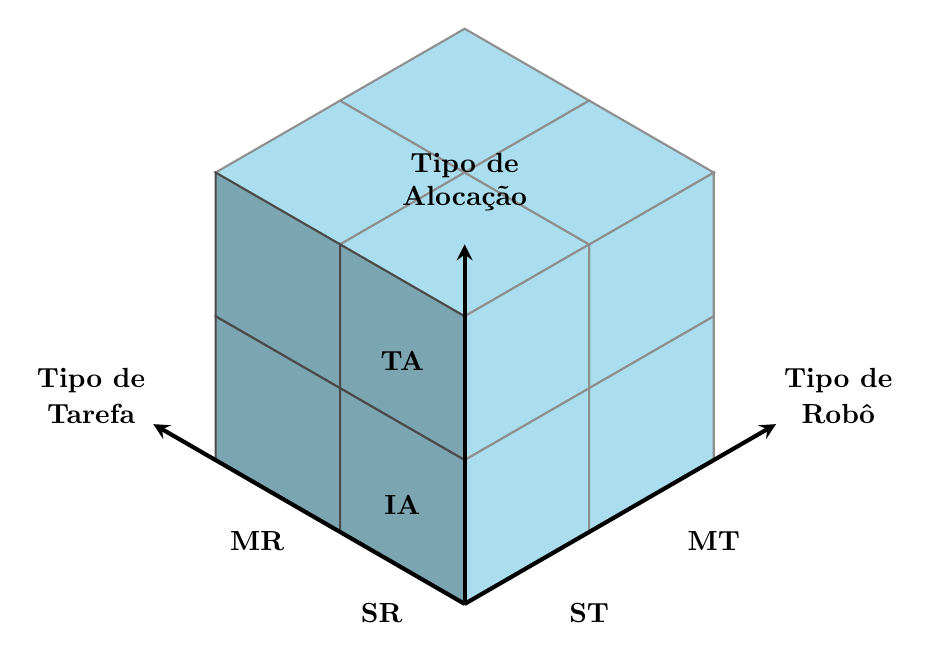
\begin{tikzpicture}
\pgftransformxscale{1.000000}
\pgftransformyscale{-1.000000}
\definecolor{dialinecolor}{rgb}{0.000000, 0.000000, 0.000000}
\pgfsetstrokecolor{dialinecolor}
\definecolor{dialinecolor}{rgb}{1.000000, 1.000000, 1.000000}
\pgfsetfillcolor{dialinecolor}
\pgfsetlinewidth{0.050000\du}
\pgfsetdash{}{0pt}
\pgfsetdash{}{0pt}
\pgfsetmiterjoin
\pgfsetbuttcap
\definecolor{dialinecolor}{rgb}{0.666667, 0.870588, 0.937255}
\pgfsetfillcolor{dialinecolor}
\fill (-5.500000\du,-10.392300\du)--(-2.500000\du,-8.660250\du)--(0.500000\du,-10.392300\du)--(-2.500000\du,-12.124400\du)--cycle;
\definecolor{dialinecolor}{rgb}{0.556863, 0.556863, 0.556863}
\pgfsetstrokecolor{dialinecolor}
\draw (-5.500000\du,-10.392300\du)--(-2.500000\du,-8.660250\du)--(0.500000\du,-10.392300\du)--(-2.500000\du,-12.124400\du)--cycle;
\pgfsetlinewidth{0.050000\du}
\pgfsetdash{}{0pt}
\pgfsetdash{}{0pt}
\pgfsetmiterjoin
\pgfsetbuttcap
\definecolor{dialinecolor}{rgb}{0.666667, 0.870588, 0.937255}
\pgfsetfillcolor{dialinecolor}
\fill (-2.500000\du,-12.124400\du)--(0.500000\du,-10.392300\du)--(3.500000\du,-12.124400\du)--(0.500000\du,-13.856400\du)--cycle;
\definecolor{dialinecolor}{rgb}{0.556863, 0.556863, 0.556863}
\pgfsetstrokecolor{dialinecolor}
\draw (-2.500000\du,-12.124400\du)--(0.500000\du,-10.392300\du)--(3.500000\du,-12.124400\du)--(0.500000\du,-13.856400\du)--cycle;
\pgfsetlinewidth{0.050000\du}
\pgfsetdash{}{0pt}
\pgfsetdash{}{0pt}
\pgfsetmiterjoin
\pgfsetbuttcap
\definecolor{dialinecolor}{rgb}{0.666667, 0.870588, 0.937255}
\pgfsetfillcolor{dialinecolor}
\fill (3.500000\du,-8.660250\du)--(3.500000\du,-5.196150\du)--(6.500000\du,-6.928200\du)--(6.500000\du,-10.392300\du)--cycle;
\definecolor{dialinecolor}{rgb}{0.556863, 0.556863, 0.556863}
\pgfsetstrokecolor{dialinecolor}
\draw (3.500000\du,-8.660250\du)--(3.500000\du,-5.196150\du)--(6.500000\du,-6.928200\du)--(6.500000\du,-10.392300\du)--cycle;
\pgfsetlinewidth{0.050000\du}
\pgfsetdash{}{0pt}
\pgfsetdash{}{0pt}
\pgfsetmiterjoin
\pgfsetbuttcap
\definecolor{dialinecolor}{rgb}{0.666667, 0.870588, 0.937255}
\pgfsetfillcolor{dialinecolor}
\fill (-2.500000\du,-8.660250\du)--(0.500000\du,-6.928200\du)--(3.500000\du,-8.660250\du)--(0.500000\du,-10.392300\du)--cycle;
\definecolor{dialinecolor}{rgb}{0.556863, 0.556863, 0.556863}
\pgfsetstrokecolor{dialinecolor}
\draw (-2.500000\du,-8.660250\du)--(0.500000\du,-6.928200\du)--(3.500000\du,-8.660250\du)--(0.500000\du,-10.392300\du)--cycle;
\pgfsetlinewidth{0.050000\du}
\pgfsetdash{}{0pt}
\pgfsetdash{}{0pt}
\pgfsetmiterjoin
\pgfsetbuttcap
\definecolor{dialinecolor}{rgb}{0.666667, 0.870588, 0.937255}
\pgfsetfillcolor{dialinecolor}
\fill (0.500000\du,-10.392300\du)--(3.500000\du,-8.660250\du)--(6.500000\du,-10.392300\du)--(3.500000\du,-12.124400\du)--cycle;
\definecolor{dialinecolor}{rgb}{0.556863, 0.556863, 0.556863}
\pgfsetstrokecolor{dialinecolor}
\draw (0.500000\du,-10.392300\du)--(3.500000\du,-8.660250\du)--(6.500000\du,-10.392300\du)--(3.500000\du,-12.124400\du)--cycle;
\pgfsetlinewidth{0.050000\du}
\pgfsetdash{}{0pt}
\pgfsetdash{}{0pt}
\pgfsetmiterjoin
\pgfsetbuttcap
\definecolor{dialinecolor}{rgb}{0.666667, 0.870588, 0.937255}
\pgfsetfillcolor{dialinecolor}
\fill (0.500000\du,-6.928200\du)--(0.500000\du,-3.464100\du)--(3.500000\du,-5.196150\du)--(3.500000\du,-8.660250\du)--cycle;
\definecolor{dialinecolor}{rgb}{0.556863, 0.556863, 0.556863}
\pgfsetstrokecolor{dialinecolor}
\draw (0.500000\du,-6.928200\du)--(0.500000\du,-3.464100\du)--(3.500000\du,-5.196150\du)--(3.500000\du,-8.660250\du)--cycle;
\pgfsetlinewidth{0.050000\du}
\pgfsetdash{}{0pt}
\pgfsetdash{}{0pt}
\pgfsetmiterjoin
\pgfsetbuttcap
\definecolor{dialinecolor}{rgb}{0.666667, 0.870588, 0.937255}
\pgfsetfillcolor{dialinecolor}
\fill (0.500000\du,-3.464100\du)--(0.500000\du,0.000000\du)--(3.500000\du,-1.732050\du)--(3.500000\du,-5.196150\du)--cycle;
\definecolor{dialinecolor}{rgb}{0.556863, 0.556863, 0.556863}
\pgfsetstrokecolor{dialinecolor}
\draw (0.500000\du,-3.464100\du)--(0.500000\du,0.000000\du)--(3.500000\du,-1.732050\du)--(3.500000\du,-5.196150\du)--cycle;
\pgfsetlinewidth{0.050000\du}
\pgfsetdash{}{0pt}
\pgfsetdash{}{0pt}
\pgfsetmiterjoin
\pgfsetbuttcap
\definecolor{dialinecolor}{rgb}{0.666667, 0.870588, 0.937255}
\pgfsetfillcolor{dialinecolor}
\fill (3.500000\du,-5.196150\du)--(3.500000\du,-1.732050\du)--(6.500000\du,-3.464100\du)--(6.500000\du,-6.928200\du)--cycle;
\definecolor{dialinecolor}{rgb}{0.556863, 0.556863, 0.556863}
\pgfsetstrokecolor{dialinecolor}
\draw (3.500000\du,-5.196150\du)--(3.500000\du,-1.732050\du)--(6.500000\du,-3.464100\du)--(6.500000\du,-6.928200\du)--cycle;
\pgfsetlinewidth{0.050000\du}
\pgfsetdash{}{0pt}
\pgfsetdash{}{0pt}
\pgfsetmiterjoin
\pgfsetbuttcap
\definecolor{dialinecolor}{rgb}{0.486275, 0.647059, 0.698039}
\pgfsetfillcolor{dialinecolor}
\fill (-2.500000\du,-8.660250\du)--(-2.500000\du,-5.196150\du)--(-5.500000\du,-6.928200\du)--(-5.500000\du,-10.392300\du)--cycle;
\definecolor{dialinecolor}{rgb}{0.290196, 0.290196, 0.290196}
\pgfsetstrokecolor{dialinecolor}
\draw (-2.500000\du,-8.660250\du)--(-2.500000\du,-5.196150\du)--(-5.500000\du,-6.928200\du)--(-5.500000\du,-10.392300\du)--cycle;
\pgfsetlinewidth{0.050000\du}
\pgfsetdash{}{0pt}
\pgfsetdash{}{0pt}
\pgfsetmiterjoin
\pgfsetbuttcap
\definecolor{dialinecolor}{rgb}{0.486275, 0.647059, 0.698039}
\pgfsetfillcolor{dialinecolor}
\fill (0.500000\du,-6.928200\du)--(0.500000\du,-3.464100\du)--(-2.500000\du,-5.196150\du)--(-2.500000\du,-8.660250\du)--cycle;
\definecolor{dialinecolor}{rgb}{0.290196, 0.290196, 0.290196}
\pgfsetstrokecolor{dialinecolor}
\draw (0.500000\du,-6.928200\du)--(0.500000\du,-3.464100\du)--(-2.500000\du,-5.196150\du)--(-2.500000\du,-8.660250\du)--cycle;
\pgfsetlinewidth{0.050000\du}
\pgfsetdash{}{0pt}
\pgfsetdash{}{0pt}
\pgfsetmiterjoin
\pgfsetbuttcap
\definecolor{dialinecolor}{rgb}{0.486275, 0.647059, 0.698039}
\pgfsetfillcolor{dialinecolor}
\fill (-2.500000\du,-5.196150\du)--(-2.500000\du,-1.732050\du)--(-5.500000\du,-3.464100\du)--(-5.500000\du,-6.928200\du)--cycle;
\definecolor{dialinecolor}{rgb}{0.290196, 0.290196, 0.290196}
\pgfsetstrokecolor{dialinecolor}
\draw (-2.500000\du,-5.196150\du)--(-2.500000\du,-1.732050\du)--(-5.500000\du,-3.464100\du)--(-5.500000\du,-6.928200\du)--cycle;
\pgfsetlinewidth{0.050000\du}
\pgfsetdash{}{0pt}
\pgfsetdash{}{0pt}
\pgfsetmiterjoin
\pgfsetbuttcap
\definecolor{dialinecolor}{rgb}{0.486275, 0.647059, 0.698039}
\pgfsetfillcolor{dialinecolor}
\fill (0.500000\du,-3.464100\du)--(0.500000\du,0.000000\du)--(-2.500000\du,-1.732050\du)--(-2.500000\du,-5.196150\du)--cycle;
\definecolor{dialinecolor}{rgb}{0.290196, 0.290196, 0.290196}
\pgfsetstrokecolor{dialinecolor}
\draw (0.500000\du,-3.464100\du)--(0.500000\du,0.000000\du)--(-2.500000\du,-1.732050\du)--(-2.500000\du,-5.196150\du)--cycle;
% setfont left to latex
\definecolor{dialinecolor}{rgb}{0.000000, 0.000000, 0.000000}
\pgfsetstrokecolor{dialinecolor}
\node at (-8.500000\du,-5.374900\du){\textbf{Tipo de}};
% setfont left to latex
\definecolor{dialinecolor}{rgb}{0.000000, 0.000000, 0.000000}
\pgfsetstrokecolor{dialinecolor}
\node at (-8.500000\du,-4.574900\du){\textbf{Tarefa}};
% setfont left to latex
\definecolor{dialinecolor}{rgb}{0.000000, 0.000000, 0.000000}
\pgfsetstrokecolor{dialinecolor}
\node at (0.500000\du,-10.571050\du){\textbf{Tipo de}};
% setfont left to latex
\definecolor{dialinecolor}{rgb}{0.000000, 0.000000, 0.000000}
\pgfsetstrokecolor{dialinecolor}
\node at (0.500000\du,-9.771050\du){\textbf{Alocação}};
% setfont left to latex
\definecolor{dialinecolor}{rgb}{0.000000, 0.000000, 0.000000}
\pgfsetstrokecolor{dialinecolor}
\node at (9.500000\du,-5.374900\du){\textbf{Tipo de}};
% setfont left to latex
\definecolor{dialinecolor}{rgb}{0.000000, 0.000000, 0.000000}
\pgfsetstrokecolor{dialinecolor}
\node at (9.500000\du,-4.574900\du){\textbf{Robô}};
\pgfsetlinewidth{0.100000\du}
\pgfsetdash{}{0pt}
\pgfsetdash{}{0pt}
\pgfsetbuttcap
{
\definecolor{dialinecolor}{rgb}{0.000000, 0.000000, 0.000000}
\pgfsetfillcolor{dialinecolor}
% was here!!!
\pgfsetarrowsstart{stealth}
\definecolor{dialinecolor}{rgb}{0.000000, 0.000000, 0.000000}
\pgfsetstrokecolor{dialinecolor}
\draw (8.000000\du,-4.330130\du)--(0.500000\du,0.000000\du);
}
\pgfsetlinewidth{0.100000\du}
\pgfsetdash{}{0pt}
\pgfsetdash{}{0pt}
\pgfsetbuttcap
{
\definecolor{dialinecolor}{rgb}{0.000000, 0.000000, 0.000000}
\pgfsetfillcolor{dialinecolor}
% was here!!!
\pgfsetarrowsstart{stealth}
\definecolor{dialinecolor}{rgb}{0.000000, 0.000000, 0.000000}
\pgfsetstrokecolor{dialinecolor}
\draw (-7.000000\du,-4.330130\du)--(0.500000\du,0.000000\du);
}
% setfont left to latex
\definecolor{dialinecolor}{rgb}{0.000000, 0.000000, 0.000000}
\pgfsetstrokecolor{dialinecolor}
\node at (-4.500000\du,-1.510800\du){\textbf{MR}};
% setfont left to latex
\definecolor{dialinecolor}{rgb}{0.000000, 0.000000, 0.000000}
\pgfsetstrokecolor{dialinecolor}
\node at (-1.500000\du,0.221250\du){\textbf{SR}};
% setfont left to latex
\definecolor{dialinecolor}{rgb}{0.000000, 0.000000, 0.000000}
\pgfsetstrokecolor{dialinecolor}
\node at (3.500000\du,0.221250\du){\textbf{ST}};
% setfont left to latex
\definecolor{dialinecolor}{rgb}{0.000000, 0.000000, 0.000000}
\pgfsetstrokecolor{dialinecolor}
\node at (6.500000\du,-1.510800\du){\textbf{MT}};
% setfont left to latex
\definecolor{dialinecolor}{rgb}{0.000000, 0.000000, 0.000000}
\pgfsetstrokecolor{dialinecolor}
\node at (-1.000000\du,-5.840930\du){\textbf{TA}};
% setfont left to latex
\definecolor{dialinecolor}{rgb}{0.000000, 0.000000, 0.000000}
\pgfsetstrokecolor{dialinecolor}
\node at (-1.000000\du,-2.376830\du){\textbf{IA}};
\pgfsetlinewidth{0.100000\du}
\pgfsetdash{}{0pt}
\pgfsetdash{}{0pt}
\pgfsetbuttcap
{
\definecolor{dialinecolor}{rgb}{0.000000, 0.000000, 0.000000}
\pgfsetfillcolor{dialinecolor}
% was here!!!
\pgfsetarrowsstart{stealth}
\definecolor{dialinecolor}{rgb}{0.000000, 0.000000, 0.000000}
\pgfsetstrokecolor{dialinecolor}
\draw (0.500000\du,-8.660250\du)--(0.500000\du,0.000000\du);
}
\end{tikzpicture}

            \caption{Representação visual da taxonomia de três eixos sugerida por \cite{ref:gerkey2004taxonomy}.} \label{fig:taxomia_mrta}
        \end{figure}
        
        É visto na Figura \ref{fig:taxomia_mrta} uma representação gráfica da taxonomia de \cite{ref:gerkey2004taxonomy} para a classificação de problemas MRTA (\textit{Multi-Robot Task Allocation}), onde pode-se notar que existem oito problemas MRTA bem definidos.
        
        \emph{\color{red} dar exemplo}
        
        \emph{\color{red} definir o escopo de problemas considerados neste trabalho}
    
    % 3a seção do capítulo 3
    \section{Arquiteturas} \label{sec:sec3_3}
        Colocar texto aqui
    
        % 1a sub-seção da 3a seção do capítulo 3
        \subsection{ALLIANCE} \label{sub:sub3_3_1}
        
            Esta é uma arquitetura totalmente distribuída, tolerante à falhas, que visa atingir controle cooperativo e atender os requisitos de uma missão à ser desempenhada por um grupo de robôs heterogêneos \cite{ref:parker1998alliance}. Cada robô é modelado usando uma aproximação baseada em comportamentos. A partir do estado do ambiente e dos outros robôs cooperadores, uma configuração de comportamento é selecionada conforme sua respectiva função de realização de tarefa na camada de alto nível de abstração. Cada configuração de comportamento permite controlar os atuadores do robô em questão de um modo diferente.
            
            Sejam $R=\{r_1, r_2, \cdots, r\}$, o conjunto de $n$ robôs heterogêneos, e $A=\{a_1,a_2, \cdots,\allowbreak a_m\}$, o conjunto de $m$ subtarefas independentes que compõem uma dada missão. Na arquitetura ALLIANCE, cada robô $r_i$ possui um conjunto de $p$ configurações de comportamento, dado por $C=\{c_{i1}, c_{i2},\cdots, c_{ip}\}$. Cada configuração de comportamento fornece ao seu robô uma função de realização de tarefa em alto nível, conforme definido em \cite{ref:brooks1986robust}. 
            
            \textbf{melhorar esse parágrafo} Além disso, o conjunto de $n$ funções $H_k=\{h_1(c_{1k}),\allowbreak h_2(c_{2k}), \cdots, h_n(c_{nk})\}$, em que $h_i(c_{ik})$ é uma função que retorna a tarefa em $A$ que o robô $r_i$ executa quando sua configuração de ativação $c_{ik}$ é ativada.
            
            A seguir, serão discutidas as funções necessárias para a ativação de uma dada configuração de comportamento $c_{ij}$ do robô $r_i$ para a execução da tarefa $h_i(c_{ij})$.
            
            \begin{equation}
                aplic\acute{a}vel_{ij}(t) =
                \begin{cases}
                    1 & \parbox[t]{.5\textwidth}{se o módulo de \textit{feedback} sensorial da configuração de comportamento $c_{ij}$ do robô $r_i$ indicar que esta configuração é aplicável mediante ao estado atual do ambiente no instante $t$;} \\
                    0 & \text{caso contrário.}
                \end{cases}
            \end{equation}
            
            \begin{equation}
                recebida_{ij}(k, t_1, t_2) =
                \begin{cases}
                    1 & \parbox[t]{.5\textwidth}{se o robô $r_i$ recebeu mensagem do robô $r_k$ referente à tarefa $h_i(c_{ij})$ dentro do intervalo de tempo $(t_1, t_2)$, em que $t_1 < t_2$;} \\
                    0 & \text{caso contrário.}
                \end{cases}
            \end{equation}
            
            \begin{equation}
                inibida_{ij}(t) =
                \begin{cases}
                    1 & \parbox[t]{.5\textwidth}{se outra configuração de comportamento $c_{ik}$ (com $k \neq j$) está ativa no robô $r_i$ no instante $t$;} \\
                    0 & \text{caso contrário.}
                \end{cases}
            \end{equation}
            
            \begin{equation}
                impaci\hat{e}ncia_{ij}(t) =
                \begin{cases}
                    \min\limits_{x}\delta_{slow_{ij}}(x, t) & \parbox[t]{.5\textwidth}{se $ recebida_{ij}(x, t - \tau_i, t) \, \land \, \lnot recebida_{ij}(x, 0, t - \phi_{ij}(x, t))$;} \\
                    \delta_{fast_{ij}}(t) & \text{caso contrário.}
                \end{cases}
            \end{equation}
            
            \begin{equation}
                reiniciada_{ij}(t) =
                \begin{cases}
                    1 & \parbox[t]{.5\textwidth}{se $\exists x, recebida_{ij}(x, t - dt, t) \: \land \: \lnot recebida_{ij}(x, 0, t - dt))$, onde $dt$ é o tempo desde a última verificação de comunicação;} \\
                    0 & \text{caso contrário.}
                \end{cases}
            \end{equation}
            
            \begin{equation}
                ativa_{ij}(\Delta t, t) =
                \begin{cases}
                    1 & \parbox[t]{.5\textwidth}{se a configuração de comportamento $c_{ij}$ do robô $r_i$ estiver ativa por mais de $\Delta t$ unidades de tempo no instante $t$;} \\
                    0 & \text{caso contrário.}
                \end{cases}
            \end{equation}
            
            \begin{equation}
                aquiescente_{ij}(t) =
                \begin{cases}
                    1 & \parbox[t]{.5\textwidth}{se $(ativa_{ij}(\psi_{ij}(t), t) \, 
                    \land \, \exists x, recebida_{ij}(x, t - \tau_i, t)) \, \lor \, ativa_{ij}(\lambda_{ij}(t), t)$;} \\
                    0 & \text{caso contrário.}
                \end{cases}
            \end{equation}
            
            \begin{equation}
                \begin{aligned}
                    motiva\textit{ç}\tilde{a}o_{ij}(0) = \ & 0 \\
                    motiva\textit{ç}\tilde{a}o_{ij}(t) = \ & (motiva\textit{ç}\tilde{a}o_{ij}(t - \delta t) + impaci\hat{e}ncia_{ij}(t)) \\
                    & \times aplic\acute{a}vel_{ij}(t) \times inibida_{ij}(t) \\
                    & \times reiniciada_{ij}(t) \times aquiescente_{ij}(t).
                \end{aligned}
            \end{equation}
            
            \pgfplotstableread[col sep=comma]{\detokenize{Figuras/capitulo_3/robot1-wander-motivation-new.csv}}\datatable
            \begin{figure}[htb]
                \centering
                \begin{tikzpicture}
    \begin{groupplot}[
      group style={rows=6}, 
      width=0.75\textwidth,
      height=0.25\textwidth, 
      xmajorgrids, 
      ymajorgrids, 
      enlarge x limits=false,
    ] 
        \nextgroupplot[
        %title={Motivação da configuração de comportamento /robot1/wander.},
        ymin=-0.1,
        ylabel={$impaci\hat{e}ncia(t)$},
        ]
        \addplot[blue,line width=1pt] table[x index=0,y index=1]{\datatable}; 
        
        \nextgroupplot[
        ymin=-0.1,
        ymax=1.1,
        ylabel={$aquiescente(t)$},
        ] 
        \addplot[blue,line width=1pt] table[x index=0,y index=2]{\datatable}; 
        
        \nextgroupplot[
        ymin=-0.1,
        ymax=1.1,
        ylabel={$inibida(t)$},
        ] 
        \addplot[blue,line width=1pt] table[x index=0,y index=3]{\datatable}; 
        
        \nextgroupplot[
        ymin=-0.1,
        ymax=1.1,
        ylabel={$reiniciada(t)$},
        ] 
        \addplot[blue,line width=1pt] table[x index=0,y index=4]{\datatable}; 
        
        \nextgroupplot[
        ymin=-0.1,
        ymax=1.1,
        ylabel={$aplic\acute{a}vel(t)$},
        ] 
        \addplot[blue,line width=1pt] table[x index=0,y index=5]{\datatable};
        
        \nextgroupplot[
        ylabel={$motiva\textit{ç}\tilde{a}o(t)$},
        xlabel={$t [s]$}
        ] 
        \addplot[blue,line width=1pt] table[x index=0,y index=6]{\datatable};
    \end{groupplot}
\end{tikzpicture}
                \caption{Motivação da configuração de comportamento /robot1/wander.} \label{fig:motivacao}
            \end{figure}